%! Author = itgramic
%! Date = 03.01.24

% Preamble
\chapter{Generell}
\begin{flushleft}
    Grundsätzlich verläuft der Patch auf den Test- und Produktivservern gleich ab.
    Die Services auf dem zweiten Server dürfen erst gestoppt werden, wenn der \Gls{JBoss}-Service auf dem ersten Server vollständig einsatzbereit ist und
    verbindungen annimmt.
\end{flushleft}
\begin{flushleft}
    Es gibt leider keine Garantie dafür, das die \Gls{JBoss}-Services laufen, wenn der Windows-Service läuft.
    Um zu Prüfen, ob der \Gls{JBoss}-Service an sich lauffähig ist, gibt es mehrere Indikatoren.
\end{flushleft}
\begin{flushleft}
    Zum einen gibt es im standalone-Verzeichnis das Subverzeichnis deployments in welchem gewisse Files auskunft über die Gesundheit des Nodes geben.
    Diese sind wie folgt zu finden:
    \dirtree{%
        .1 /.
        .2 laufwerk.
        .3 phoenix-server-<system>-<version>.
        .4 <node>.
        .5 standalone.
        .6 deployments.
    }
\end{flushleft}
\begin{flushleft}
    Bei einem geglückten Deployment eines Nodes muss ein \textit{phoenix.ear}- und \textit{phoenix.ear.deployed}-File vorhanden sein.\\Bei einem Fehler wiederum wird i.d.R. \textit{phoenix.ear.failed}-File erzeugt.
    \begin{figure}[H]
        \centering
        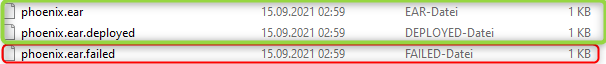
\includegraphics[width=1\linewidth]{source/general/deployments}
        \caption{Deployment-Status}
        \label{fig:deployment-status}
    \end{figure}
    Das entsprechende Mail ist im Anhang in folgendem Kapitel zu finden: \autoref{chap:811534244}
\end{flushleft}
\begin{flushleft}
    Allerdings ist dies nicht immer 100\% verlässlich.
    Die sicherste Methode, um die Funktionsfähigkeit eines Nodes resp.
    Servers zu testen besteht darin, die \textit{Workstation.exe} nur noch auf den entsprechenden Node resp.
    Server verbinden zu lassen.
    Die Verbindung wird ins \textit{Workstation.ini} geschrieben, welches wie üblich hier zu finden ist:
\end{flushleft}
\begin{flushleft}
    \dirtree{%
        .1 /.
        .2 C:\textbackslash.
        .3 Program Files (x86).
        .4 <Phoenix7-Verzeichnis>.
        .5 Workstation.ini.
    }
\end{flushleft}
\begin{flushleft}
    Im Ini stehen die \Gls{JBoss}-Server und Nodes im Eintrag \textit{-Dphoenix.server.nodes}.
    Hier das Beispiel des Produktiven Ini-Files:
    \lstset{style=gra_codestyle}
    \begin{lstlisting}[language=sh, caption=Workstation.ini PROD Beispiel,captionpos=b,label={lst:workstation.ini-prod-beispiel},breaklines=true]
    -clean
    -data
    @noDefault
    -configuration c:/temp/phoenix/prod_7_23_1/eclipse/configuration
    -nl
    de_CH
    -vmargs
    -Dorg.eclipse.update.reconcile=false
    -Dphoenix.db=Phoenix
    -Dphoenix.application.workspace.createdir=true
    -Dphoenix.application.workspace=\\\\phoenix\workspace\prod_7_23_1
    -Dphoenix.login.usernamefile=%APPDATA%/Phoenix/login_username_prod
    -Dphoenix.server.nodes=sks0020:8443,sks0021:8443,sks0020:8543,sks0021:8543
    -Djavax.net.ssl.trustStore=C:\Program Files (x86)\Phoenix7\truststore.jks
    -Dphoenix.login.enableLDAP=true
    -Dphoenix.application.winlogin=true
    -XX:-CreateMinidumpOnCrash
    \end{lstlisting}
\end{flushleft}
\begin{flushleft}
    Erkennen, ob ein \Gls{JBoss}-Service gestoppt ist, tut man daran, dass folgender Eintrag zuletzt im \texttt{server.log} steht:
    \lstset{style=gra_codestyle}
    \begin{lstlisting}[language=sh, caption=Service gestoppt - server.log,captionpos=b,label={lst:service-stopped-service.log},breaklines=true]
2024-01-05 10:56:10,422 INFO  [--] [org.jboss.as] ip[] mib[] user[] session[] request[] thread[MSC service thread 1-3]: WFLYSRV0050: JBoss EAP 7.4.8.GA (WildFly Core 15.0.19.Final-redhat-00001) stopped in 1199ms
    \end{lstlisting}
    Ein Erfolgreicher start erkennt man wiederum an folgenden Eintrag:
    \lstset{style=gra_codestyle}
    \begin{lstlisting}[language=sh, caption=Service gestartet - server.log,captionpos=b,label={lst:service-started-service.log},breaklines=true]
2024-01-05 11:01:36,000 INFO  [--] [com.cgm.phoenix.common.masterdata.srv.catalog.dao.CatalogValueDAO] ip[] mib[] user[] session[] request[] thread[ServerService Thread Pool -- 273]: Creating folder index...
2024-01-05 11:01:36,047 INFO  [--] [com.cgm.phoenix.common.masterdata.srv.catalog.dao.CatalogValueDAO] ip[] mib[] user[] session[] request[] thread[ServerService Thread Pool -- 273]: Creating search index...
2024-01-05 11:02:00,656 INFO  [--] [com.cgm.phoenix.common.masterdata.srv.catalog.dao.CatalogValueDAO] ip[] mib[] user[] session[] request[] thread[ServerService Thread Pool -- 273]: Catalog data loaded.
2024-01-05 11:02:00,656 INFO  [--] [com.cgm.phoenix.common.masterdata.srv.catalog.CatalogCacheProvider] ip[] mib[] user[] session[] request[] thread[ServerService Thread Pool -- 273]: Instant Catalogs successfully initialized.
2024-01-05 11:02:00,891 INFO  [--] [org.jboss.as.server] ip[] mib[] user[] session[] request[] thread[ServerService Thread Pool -- 43]: WFLYSRV0010: Deployed "phoenix.ear" (runtime-name : "phoenix.ear")
2024-01-05 11:02:00,891 INFO  [--] [org.jboss.as.server] ip[] mib[] user[] session[] request[] thread[ServerService Thread Pool -- 43]: WFLYSRV0010: Deployed "jolokia.war" (runtime-name : "jolokia.war")
2024-01-05 11:02:00,922 INFO  [--] [org.jboss.as.server] ip[] mib[] user[] session[] request[] thread[Controller Boot Thread]: WFLYSRV0212: Resuming server
2024-01-05 11:02:01,000 INFO  [--] [org.jboss.as] ip[] mib[] user[] session[] request[] thread[Controller Boot Thread]: WFLYSRV0025: JBoss EAP 7.4.8.GA (WildFly Core 15.0.19.Final-redhat-00001) started in 281140ms - Started 18250 of 18473 services (563 services are lazy, passive or on-demand)
2024-01-05 11:02:01,000 INFO  [--] [org.jboss.as] ip[] mib[] user[] session[] request[] thread[Controller Boot Thread]: WFLYSRV0060: Http management interface listening on http://10.0.22.52:9990/management
2024-01-05 11:02:01,016 INFO  [--] [org.jboss.as] ip[] mib[] user[] session[] request[] thread[Controller Boot Thread]: WFLYSRV0051: Admin console listening on http://10.0.22.52:9990
    \end{lstlisting}

    Es kann aber mehrere Minuten dauern, bis ein Service vollständig gestartet ist.
\end{flushleft}
\begin{flushleft}
    Am Einfachsten ist, man erstellt sich drei Ini-Files, eines für beide Server zusammen im Cluster und eines pro Server.
    Dann braucht man nur die Files umzubennen und kann rasch Testen.
\end{flushleft}
\begin{flushleft}
    \begin{mdframed}
    Vorsichht!\\Es kann vorkommen, dass jeder Server für sich alleine Lauffähig ist aber im Cluster-Verbund keine Anmeldung möglich ist!\\
    Daher sollte nach einem Reboot nebst der Lauffähigkeit der einzelnen Nodes auch immer der Cluster getestet werden!
    \end{mdframed}
\end{flushleft}
\begin{flushleft}
    Obwohl die Server mittels \Gls{Ivanti} betankt werden, kann es vorkommen, dass nicht alle Patches geladen wurden.
    Um sicherzustellen, dass das System komplett sauber gepatched wurde, sollte man immer noch auf Updates Prüfen.

    Geprüft wird Normal via Suche:
    \begin{figure}[H]
        \centering
        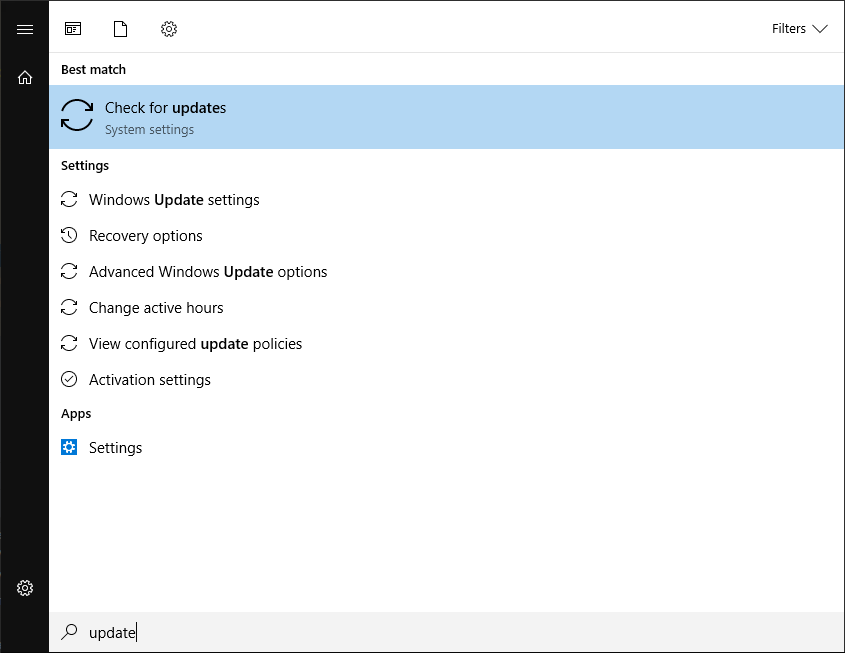
\includegraphics[width=1\linewidth]{source/general/search_for_updates}
        \caption{Check-Updates}
        \label{fig:check-updates}
    \end{figure}

    \begin{mdframed}
    Wurde der Server von Ivanti korrekt betankt, so sind meistens zwei Patches vorhanden bei denen \texttt{Restart required} steht.
    \end{mdframed}

    Solange noch Updates wie folgt, vorhanden sind, müssen diese manuell nachgeladen und installiert werden:
    \begin{figure}[H]
        \centering
        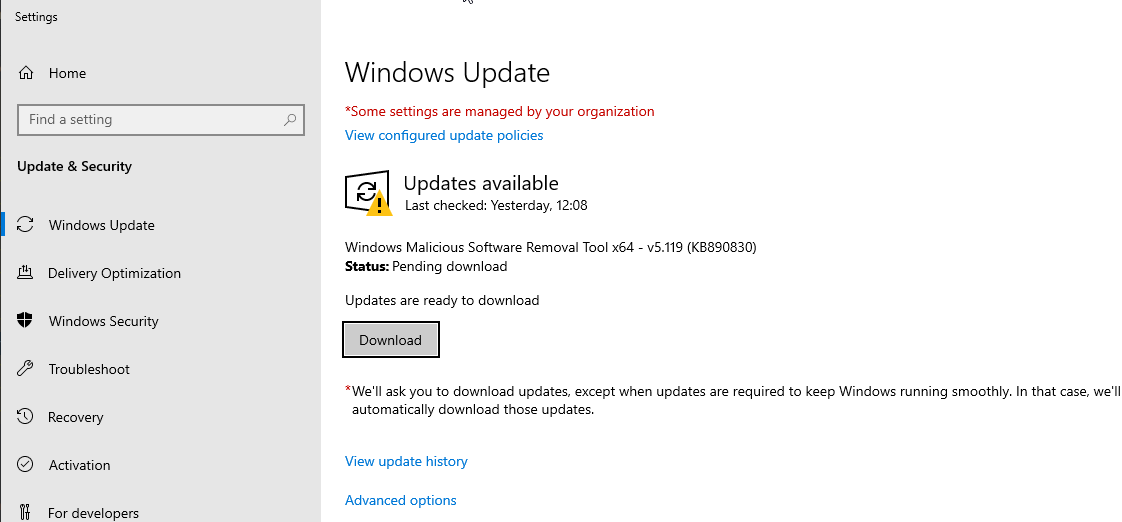
\includegraphics[width=1\linewidth]{source/general/updates_available}
        \caption{Updates available}
        \label{fig:updates-available}
    \end{figure}

    Dies ist aber äusserst selten der Fall.

    \begin{mdframed}
    Vorsichht!\\Sollte es trotzdem mal vorkommen, niemals die \Gls{RDP}-Verbindung schliessen!\\Ansonsten wird es unmöglich sein, den Server gezielt zu rebooten.
    \end{mdframed}
\end{flushleft}
\begin{flushleft}
    Desweiteren muss auf der \Gls{VMware vSphere} die Berechtigung gegeben sein, Snapshots erstellen und löschen zu können.
    Auch Restores via Snapshot sollten machbar sein.
\end{flushleft}